\documentclass{article}
\usepackage[utf8]{inputenc}

\usepackage{natbib}
\usepackage{graphicx}
\usepackage[]{hyperref}
\usepackage[]{physics}
\usepackage[]{listings}
\usepackage[T1]{fontenc}
\usepackage{color}

\lstset{
  backgroundcolor=\color{white}, % requires \usepackage{color} or \usepackage{xcolor}
  basicstyle=\footnotesize,
  breakatwhitespace=false,
  breaklines=true,
  captionpos=b,
  commentstyle=\color{green},
  deletekeywords={...},
  escapeinside={\%*}{*)},
  extendedchars=true,
  frame=single,
  keepspaces=true,
  keywordstyle=\color{blue},
  language=c++,
  otherkeywords={*,...},
  rulecolor=\color{black},
  showspaces=false,
  showstringspaces=false,
  showtabs=false,
  stepnumber=2,
  %stringstyle=\color{pink},
  tabsize=4,
}

\title{Solving the 1-dimentional Poisson equeation}
\author{
  Brandt, Samuel\\
 % \texttt{}
  \and
  Davidov, Aleksandar\\
  \textcolor{blue}{\href{https://github.com/aleksda/FYS4150/}{\texttt{github.com/aleksda}}}
  \and
  Hemaz, Said\\
  % \texttt{first2.last2@xxxxx.com}
}
\date{September 2019}

\begin{document}

\maketitle
\begin{abstract}
The objective of this project is to solve the one dimensional version of the Poisson equation with Dirichlet boundary condition, using two different algorithms. The problem can be formulated as a set of linear equations because of its discretized nature.  Furthermore a determination of which of the algorithms is more effective at solving the equation is going to be made. In this case the two algorithms will be TDMA (tridiagonal matrix method) and LU decomposition.

\end{abstract}
\tableofcontents

\iffalse
\begin{figure}[h!]
\centering
\includegraphics[scale=1.7]{universe}
\caption{The Universe}
\label{fig:universe}
\end{figure}
\fi
\newpage

\section{Introduction}
As they say " the language of physics is math" , this could not ring anymore true, since all the problems we have in physics can be broken down to some form of a mathematical equation(s). In particular differential equations is more widely used to explain the physical world. They say something about how the rates of changes in a given system occurs. The advances in technology have made it possible for us to solve these equations with incredible power, as the analytic solutions can have their limitations. These forms of solutions is also known as numerical solutions, an can be solves within seconds using a computer. \\

The purpose of this task is to explore a set of differential equations, known as one-dimensional Poisson's equation with Dirichlet boundary conditions. Even further are we going to explore the different numerical tools we have, and which one will be more efficient in terms of time. Since we are dealing with a set of equations, linear algebraic method like TMA and LU decomposition will be more appropriate to explore. 

\section{Theory}
\subsection{Second-order Differential Equations}

In science, there are many important algorithms that can be be written as a linear second-order differential equation. These equation are on the form
$$\frac{d^{2}y}{dx^{2}} + g(x)y(x) = f(x)$$
where $g(x)$ and $y(x)$ are real function, while $f(x)$ is the inhomogeneous term.
\newline
\subsection{The Poisson Equation} 

\newline The equation we will study in this article is a widely used differential equation in physics and other fields, namely the Poisson's Equation.
\begin{equation}
    \laplacian \Phi = -4 \pi \rho(\vb{r}) % From physics library
\end{equation}
Here, we have the electrostatic potential $\Phi$ that is generated by the localized charge distribution given by $\rho(\vb{r})$.
\newline
If we would consider spherical symmetry for for the potential, $\Phi$, and the charge distribution, $\rho(\vb{r})$, our equation would be simplified to the one dimensional equation
$$
    \frac{1}{r^2}\frac{d}{dr}\left( r^2 \frac{d\Phi}{dr} \right) = -4\pi\phi(r),
$$
With the substitution, $\Phi(r)=\phi(r)/r$, we can now once again rewrite our equation (1) as
$$
    \frac{d^2\phi}{dr^2} = -4\pi r \rho(r)
$$
Now, our inhomogeneous term, $f(x)$ is, as we can see, given by the constant $4\pi$ multiplied by $r$ and the charge distribution $\rho$.
\newline\newline
Once again, we can rewrite this equation further by letting $\phi \rightarrow u$ and $r \rightarrow x$. Our one-dimensional Poisson's equation will then read

\subsection{Methods for numerical solving}
In this project, the one-dimensional Poisson Equation was solved with Dirichlet boundary conditions, in the case with $$-u''(x) = f(x), \hspace{0.5cm} u(0)=u(1)=0\hspace{0.5cm} x\in(0,1)$$. The way this was done, was by rewriting it as a set of linear equations. Bellow, you will see that the discretized approximation of $u$ is given as $v_i$, and the grid points as, $x_i=ih$, where $h$ is the step length defined as $h=1/(n+1)$ on the open interval $(0,1)$ where $x_0=0$ and $x_{n+1}=1$.Finally, now we approximate the second derivative of $u$ with 
\begin{equation}
   -\frac{v_{i+1}+v_{i-1}-2v_i}{h^2} = f_i  \hspace{0.5cm} \mathrm{for} \hspace{0.1cm} i=1,\dots, n,
\end{equation}
where $f_i=f(x_i)$.
\newline
We can now rewrite (3) as a set of linear equations that we can use to solve it numerically if we rewrite it on the form
\begin{equation*}
%\begin{align*}
 {A}\textbf{x} &= \textbf{w}
%\end{align*}
\end{equation*}
where $\mathbf{A}$ is the $n \times n$ tridiagonal matrix written as

\[ % Taken as it was in the Project1.pdf file
    \mathbf{A} = \begin{bmatrix}
                           2& -1& 0 &\dots   & \dots &0 \\
                           -1 & 2 & -1 &0 &\dots &\dots \\
                           0&-1 &2 & -1 & 0 & \dots \\
                           & \dots   & \dots &\dots   &\dots & \dots \\
                           0&\dots   &  &-1 &2& -1 \\
                           0&\dots    &  & 0  &-1 & 2 \\
                      \end{bmatrix},
\]
while ${w}_i=h^2f_i$. 
\newline\newline
We can see that this holds true as (3) can be rewritten as $-v_{i+1} - 2v_i + v_{i-1}={w}_i=h^2f_i$. Now, when calculation numerically, we don't need the endpoints, since they are set by the boundary condition. Our equation can therefore be represented as ${A}\textbf{x} &= \textbf{w}


\subsection{Our problem}
In our case, we have that $f(x)=100 e^{-10x}$ with the boundary conditions specified above. With the methods discussed in the previous section, we should be able to find an approximation of $u$ with good accuracy. Even better, when we find a numerical solution, since the solution has an analytical form, we should be able compare them and test the accuracy and speed for our numerical algorithms. Our analytical closed-form solution is expressed as $$u(x)=1-(1-e^{-10})x-e^{-10x}$$

\section{Code implementation/testing}
\subsection{Tridiagonal matrix algorithm (TMA) (generalized)}
Generally speaking in linear algebra, any set of equations can be broken down to the following equation :
\begin{align*}
 {A}\textbf{x} &= \textbf{w}
\end{align*}

The solution of such equations are based on the Gaussian elimination method. This is a method which consists of a sequence of operaations performed in the rows of the matrix with the purpose of reducing it to a upper/triangular matrix in row echelon form. These operations are as follows:\\

%I) Swapping two rows
%\\II) Multiplying a row by a nonzero number
%\\III) Adding a multiple of one row to another row\\
\begin{itemize}
  \item Swapping two rows
  \item Multiplying a row by a nonzero number
  \item Adding a multiple of one row to another row
\end{itemize}

These operations are the basis of our solution, yet there are more specific methods composed of such operations, they are known as forward and backward substitution. Consider the following 4 x 4 matrix :


\begin{align*}
  \begin{bmatrix}
      b_1 & c_1 & 0   & 0   \\
      a_1 & b_2 & c_2 & 0   \\
      0   & a_2 & b_3 & c_3 \\
      0   & 0   & a_3 & b_4
  \end{bmatrix}
  \begin{bmatrix} x_1 \\ x_2 \\ x_3 \\ x_4 \end{bmatrix}
    &=
  \begin{bmatrix} w_1 \\ w_2 \\ w_3 \\ w_4 \end{bmatrix}
\end{align*}

Performing basic Gaussian elimination operations on it, will yield us a pattern for the specific methods, for forward substitution we get:
\begin{align*}
{x}_i = \frac{w_i -\sum_{j=i + 1}^{n} a_{i,j}x_{j}}    {{a}_{i,i}} \hspace{1.0cm} for\hspace{0.1cm}i=n-1, n-2,..,1
\end{align*}
In C++, the code for this algorithm look like this:
\begin{lstlisting}
// Forward substitution
// Boundary conditions
diag[1] = d[1];
f_tilde[1] = b_tilde[1];
for (int i = 2; i <= n; i++) {
    diag[i] = d[i] - ((a[i] * c[i - 1]) / diag[i - 1]);
    f_tilde[i] = b_tilde[i] - ((f_tilde[i - 1] * a[i]) / diag[i - 1]);
\end{lstlisting}
In order to make everything work, we also need an algorithm for the backwards substitution. For it, the pattern is as follows:

\begin{align*}
{x}_i = \frac{ w_i -\sum_{j=1}^{i-1} a_{i,j}x_{j}}    {{a}_{i,i}} \hspace{1.0cm} for\hspace{0.1cm}i=2, 3,..,n
\end{align*}
While in C++, the code will look something like:
\begin{lstlisting}
// Backward substitution
// Boundary condition
v[n] = f_tilde[n] / diag[n];
for (int i = n - 1; i >= 1; i--){
    v[i] = (f_tilde[i] - c[i] * v[i + 1]) / diag[i];
}
\end{lstlisting}
Since we will compare this method with a more specialized one, it is a good idea to compare their efficiency. One good way to do this is to meassure the number of Floating-Point Operations (FLOPs) each algorithm has.
\newline
As we can see, the Forward substitution algorithm requires $3 + 3 = 6$ FLOPs while iterating, and a total of $n-1$ iteration. We can see that because $n$ starts from $2$ in the for-loop. This gives a total of $6(n-1)$ FLOPs for the Forward Substitution. Together with the Backward substitution algorithm, it will require a total of $8(n-1)$ FLOPs. We can say $8n$ FLOPs for the sake of simplicity 

\subsection{Tridiagonal matrix algorithm (TMA) (specialized)}
To further improve our code, we exploit the fact that our matrix is symmetric and has the same value of 2 over the diagonal ,and the value of -1 along the diagonal below and above the main diagonal. This will simplify our equation, where  $\tilde{b}_i$ is the main diagonal elements. ${a}_i$  and ${c}_i$ will equal to -1:

\begin{align*}
  \tilde{b}_i &= 2 - \frac{1}{\tilde{b}_{i-1}} \\
\end{align*}
 Forward substitution can further be upgraded to, such that it can be done with only 2 FLOPs:\\
\begin{align*}
  \tilde{f}_i &= f^{*}_i + \frac{\tilde{f}_{i-1}}{\tilde{b}_{i-1}},  \\
\end{align*}

Though the boundary conditions  $\tilde{b}_i$ =${b}_1$ = 2 we find an analyical expression for the main diagonal , which has the solution
\begin{equation*}
\tilde{b}_1 = \frac{i+1}{i}
\end{equation*}

As for the backward substitution, the optimization looks as follows:
\begin{align*}
  {v}_i &= f^{*}_i + \frac{1}{\tilde{b}_{i-1}}(\tilde{f}_{i-1} + {v}_i)  \\
\end{align*}

In relation to forward substitutions , backward substitution also requires 2 FLOPs, making the total specialized algorithm only run on 4(n) FLOPs. This is twice the speed of the generalized algorithm.
\newline\newline
The source code is given by:
\begin{lstlisting}
// Forward substitution
f_tilde[1] = b[1];
diag[1] = d[1];
for (int i = 2; i <= n; i++) {
    diag[i] = d[i] - (1.0 / diag[i - 1]);
    f_tilde[i] = b[i] + f_tilde[i - 1] / diag[i - 1];
}
\end{lstlisting}
and
\begin{lstlisting}
// Backward substitution
v[n] = f_tilde[n] / diag[n];
for (int i = n - 1; i >= 1; i--){
    v[i] = (f_tilde[i] + v[i + 1]) / diag[i];
}
\end{lstlisting}

\subsection{LU decomposition method}

LU decomposition is a method where a non-singular matrix ${A}$ is factorized to lower triangular matrix ${L}$ and an upper triangular matrix ${U}$
\begin{align*}
  {A} &= {L}{U} \\
  \begin{bmatrix}
      a_{11} & a_{12} & a_{13}  & a_{14}   \\
      a_{21} & a_{22} & a_{23} & a_{24}   \\
      a_{31} & a_{32} & a_{33} & a_{34} \\
      a_{41} & a_{42} & a_{43} & a_{44}
  \end{bmatrix}
  &=
    \begin{bmatrix}
      1 & 0 & 0   & 0   \\
      l_{21} & 1 & 0 & 0   \\
      l_{31} & l_{32} & 1 & 0 \\
      l_{41} & l_{42} & l_{43} & 1
  \end{bmatrix}
    \begin{bmatrix}
      \tilde{u}_{11} & \tilde{u}_{12} & \tilde{u}_{13}  & \tilde{u}_{14}   \\
      0 & \tilde{u}_{22} & \tilde{u}_{23} & \tilde{u}_{24}   \\
      0   & 0 & \tilde{u}_{33} & \tilde{u}_{34} \\
      0   & 0   & 0 & \tilde{u}_{44}
  \end{bmatrix}.
\end{align*}

By writing the matrix ${A}$ as its LU decomposition, we can solve the following equation:
\begin{align*}
 {A}\textbf{x} &= \textbf{w}
\end{align*}
Into two steps:

\begin{equation}
{L}{U}\textbf{x} = \textbf{w}\leftrightarrow   {L}\textbf{y} = \textbf{w}, \quad  {U}\textbf{x} = \textbf{y}.
\end{equation}
The lower triangular equation ${L}\textbf{y} = \textbf{w}$ can be solved by forward substitution, and the other equation {U}\textbf{x} = \textbf{y} with backward substitution.\\


The approach for numerical simulations is to solve Eq. \eqref{system} with the three different algorithms. We also studied the relative error of the algorithms as function of $n$ by using Eq. \eqref{calc_deviation}. Further we compared the runtimes of the different algorithms.

$$-u''(x) = f(x)$$

\section{Analysis}
When we tested the algorithms, it was noticeable that the specialized tridiagonal matrix algorithm was the most efficient one in terms of speed. Bellow in Figure \ref{fig:time} is a plot of the speed for the specialized TMA algorithm and the LU algorithm with $n=10,100,1000,1000$ computations.
\begin{figure}[h!]
\centering
%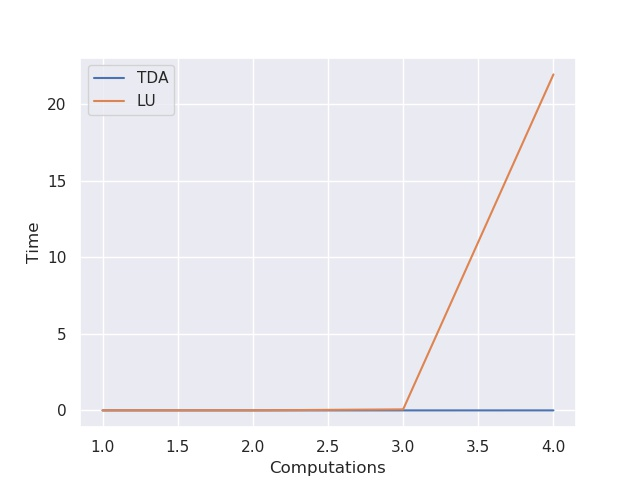
\includegraphics[scale=1.7]{time.jpg}
 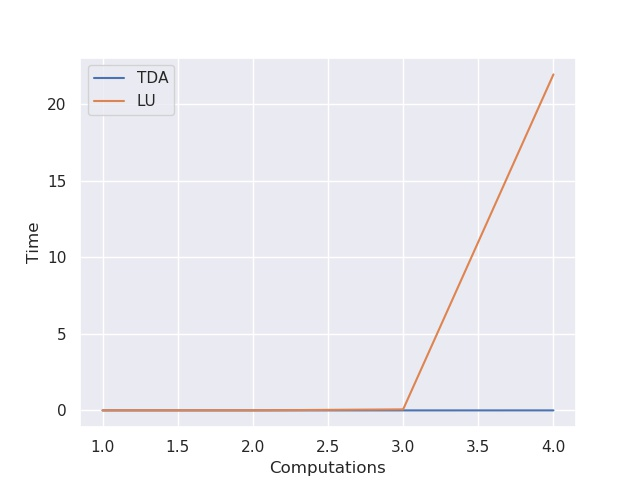
\includegraphics{time.jpg}
\caption{Time Comparison}
\label{fig:time}
\end{figure}

The LU algorithm was slower already from $n=10$, but at $n=1000$ the time it took for the LU algorithm jumped to 20 seconds. It was no point in testing it any further as the LU algorithm started to be to slow. 
\newline\newline
Now, using our algorithms to see how well they compare against the analytical solution. Bellow Figure \ref{fig:plot} is a plot for exactly that. 

\begin{figure}[h!]
\centering
%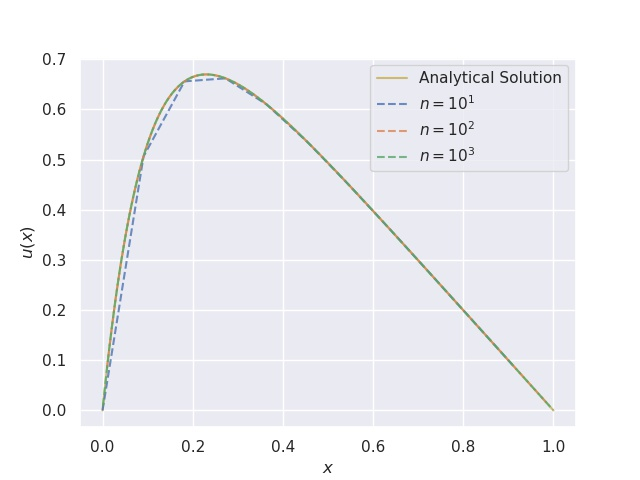
\includegraphics[scale=1.7]{plot.png}
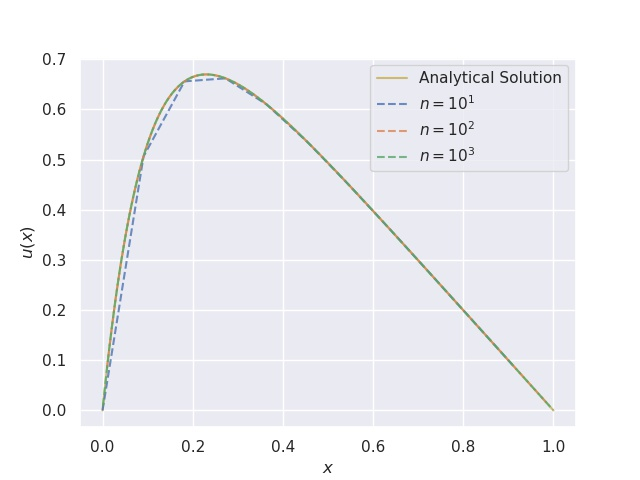
\includegraphics{plot.jpg}
\caption{Analytical vs Numerical}
\label{fig:plot}
\end{figure}

We see that the plot is from $u(0)=u(1)=0$ as was originally our problem. From the plot, it is noticeable that the numerical solution is a little inaccurate for $n=10$. However, this inaccuracy is bearly noticeable for $n=100$, and unnoticeable for $n=100$. Overall, the results seem very good.
\newline\newline
We also have a plot of the maximum relative error for the TDA algorithm in figure \ref{fig:error}. 
\begin{figure}[h!]
\centering
%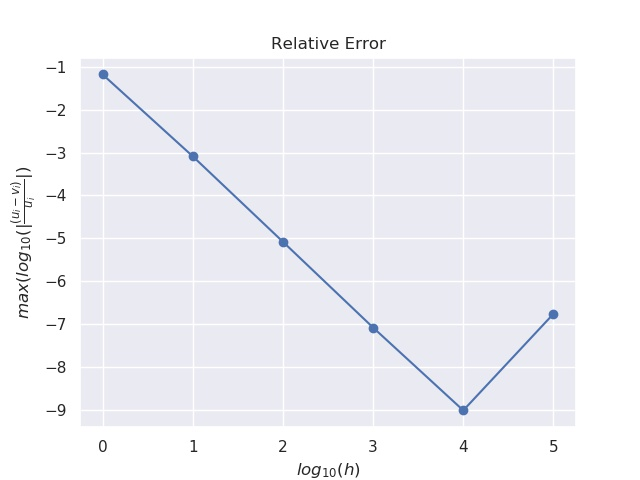
\includegraphics[scale=1.7]{error.png}
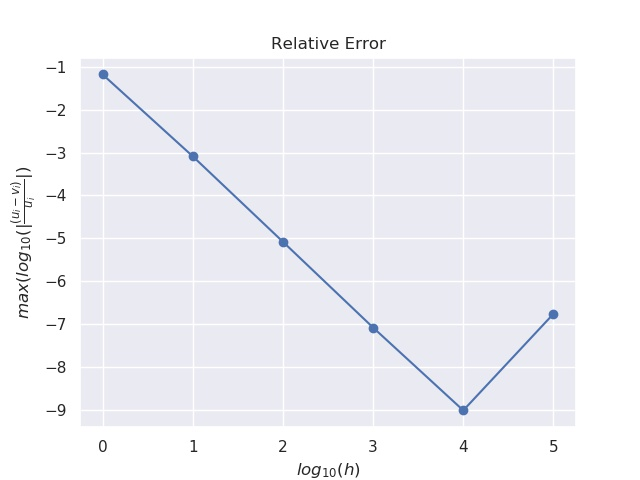
\includegraphics{error.jpg}
\caption{Relative Error}
\label{fig:error}
\end{figure}

The important part to observe here is that the error is falling with the step size until it reaches a point. After that, further falling of the step size will result in the error growing. It is uncertain why this happens. My theory is that this is happening because of loss in numerical precision when representing small values.

\section{Conclusion}
In this project we have solved the one-dimensional equation of Poisson's equation with Dirichlet boundary conditions. The function was discretized in order to make the non-linear equation solvable using linear algebraic methods. Algorithms has been programmed to solve for both the general tridiagonal matrix and the specific one for our case. For the general we had 8n FLOPs while the special case had 4(n) FLOPs, since the speed of the algorithm is proportional to the amount of FLOPs. The special one saw an increase of two times the speed of the general one. The LU decomposition method proved to be a much less preferable alternative, considering its FLOPs to be {3/2n^3}. This takes up lots of memory and time to run , which is not an ideal scenario for us looking for efficient algorithms.


\citep{CompFys2015MHJ}


%\section{Sources}
%http://mathfaculty.fullerton.edu/mathews/n2003/BackSubstitutionMod.html


\bibliographystyle{plain}
\bibliography{references}
\end{document}
